\documentclass{standalone}
\usepackage{tikz}
\begin{document}
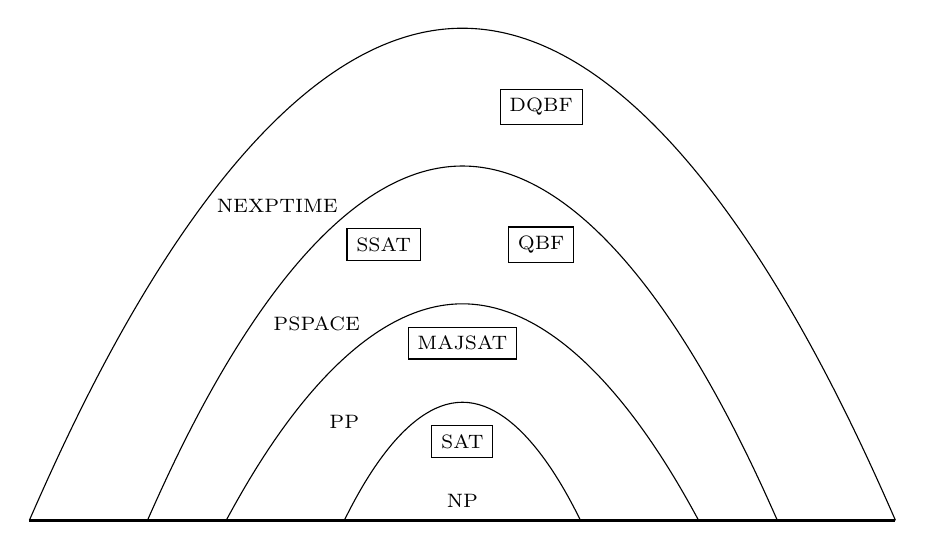
\begin{tikzpicture}
      \tikzstyle{every node}=[font=\scriptsize]
      \pgftransformscale{.5}
      %%% HELP LINES - uncomment to design/extend
      %\draw[step=1cm,gray,very thin] (-10,0) grid (10,12);
      %\node at (0,0) {\textbf{(0,0)}};
      %% Horizontal bar
      \draw[very thick] (-11,0) -- (11,0);
      % NP
      \draw (-3,0) parabola bend (0,3) (3,0);
      \node at (0,0.5) {NP};
      \node at (0,2) [draw,rectangle] {SAT};
      % PP
      \draw (-6,0) parabola bend (0,5.5) (6,0);
      \node at (-3,2.5) {PP};
      \node at (0,4.5) [draw,rectangle] {MAJSAT};
      % PSPACE
      \draw (-8,0) parabola bend (0,9) (8,0);
      \node at (-3.7,5) {PSPACE};
      \node at (2,7) [draw,rectangle] {QBF};
      \node at (-2,7) [draw,rectangle] {SSAT};
      % NEXPTIME
      \draw (-11,0) parabola bend (0,12.5) (11,0);
      \node at (-4.7,8) {NEXPTIME};
      \node at (2,10.5) [draw,rectangle] {DQBF};
\end{tikzpicture}
\end{document}